\documentclass[letterpaper, 12pt]{report}
\usepackage{enumitem, hyperref, graphicx}

\begin{document}
\title{Observatory Operations Manual}
\author{Department of Physics and Astronomy\\
	Minnesota State University Moorhead}
\maketitle
\tableofcontents
\newpage

\begin{table}[]
	\centering
	\caption{Important Phone Numbers}
	\label{tbl-phone-numbers}
	\begin{tabular}{lll}
		\hline
		Control Room    & 218 - 498 - 2930        &                           \\
		Dr. Cabanela    & 218 - 477 - 0444 (Home) & 218 - 477 - 2453 (Office) \\
		Dr. Craig       & 218 - 443 - 5979 (Cell) & 218 - 477 - 2439 (Office) \\
		Dr. Winkler     & 218 - 291 - 0853 (Home) & 218 - 477 - 2460 (Office) \\
		Campus Security & 218 - 477 - 2449        &                           \\
	\end{tabular}
\end{table}

\textbf{If you run into a technical problem that you cannot fix, remember that you can just close the dome and turn the telescope power off and you will not damage anything. Let someone know the next day.} \\

\vspace{.25in}

{\huge\textbf{In case of emergency:}}
\begin{enumerate}
	\item Call 911 and give them the Buffalo River Site address:
	\begin{itemize}
		\item [] 663 164th St. South
		\item [] Glyndon, MN 56547
	\end{itemize}
	\item Call MSUM Security (see \ref{tbl-phone-numbers})
	\item Call Dr. Cabanela, Dr. Craig, or Dr. Winkler
\end{enumerate}

\newpage

\chapter{Overview} \label{ch:1}
Using the telescope boils down to doing just a few things. Details of each of the items below are in the rest of this manual, but it is helpful have a big picture of what you will be doing before going into the details.

Note that the steps below do not necessarily have to be done in order.. It is possible to take images without turning on the telescope control system (DFM TCS, the software that steers the telescope) and it is possible to steer the telescope without the camera turned on.

The Steps:
\begin{itemize}
	\item Turn on the power to the computers, telescope, and camera. See Chapter \ref{ch:power}.
	\item Initialize the camera and telescope See Chapter \ref{ch:initialization}.
	\begin{itemize}
		\item Take darks, flats, and bias images.
		\item Initialize telescope pointing
	\end{itemize}
	\item Focus the camera and take images. See Chapters \ref{ch:focusing} and \ref{ch:shooting}.
	\item Make the Observing Log. See Chapter \ref{ch:log}
	\item Shutdown. See Chapter \ref{ch:shutdown}
	\begin{itemize}
		\item Shut down the camera
		\item Shut down the telescope
		\item Turn off all power.
	\end{itemize}
\end{itemize}

\newpage

\chapter{Power On}\label{ch:power}

\textbf{Turn off the outside lights}
\begin{itemize}
	\item In room 110, the room by the kitchen, there is a light switch that controls the outside lights. Turn off these lights, unless you like bad images
\end{itemize}

{\large\textbf{Control Room}}
\begin{itemize}
	\item \textbf{Turn on the surge protectors}
	\begin{itemize}
		\item Turn on the surge protectors on top of the Motor Driver Chassis (MDC). This is the big blue box. It is very hard to miss.
	\end{itemize}
	\item \textbf{Start the PC}
	\begin{itemize}
		\item Open the lower door on the MDC and boot the computer with the rocker switch.
		\item Close lower door.
	\end{itemize}
	\item \textbf{Turn the MDC on}
	\begin{itemize}
		\item Turn the switch labelled ``MTR DRIVER CHASSIS'' on.
	\end{itemize}
	\item \textbf{In the Dome} \\
	\noindent \textbf{The camera power supply is kept in the control room; bring it with you to the dome.}
	\begin{itemize}
		\item Plug in the camera.
		\item Attach the brick to the bottom of the telescope.
	\end{itemize}
\end{itemize}

\newpage



\chapter{Initialization}\label{ch:initialization}
\textbf{Note: This assumes that the calibration images are taken first, and not the science images. This does not have to be the case; if time is an issue based on what you are observing, calibration images can be taken later in the night. Either way, do not forget to take calibration images.} \\

\section{Initialize the telescope}


{\large\textbf{In the dome}}
\begin{itemize}
	\item Note the air temperature. It will be needed for estimating the focus.
	\item Remove the cover from the telescope. Replace it with the the light diffuser from the table. This cover is only necessary for calibration images. Remove it before starting science images.
	\item Position the lights needed for taking flats. There is a halogen light that should be placed on the step ladder and aimed at the white screen on the dome. The other is a lamp that should be clamped to the railing and also aimed at the screen.
	\item \emph{Unless you are shooting Flats, be sure to turn off the lights when exiting the dome.}
\end{itemize}

{\large\textbf{In the control room}}
\begin{itemize}
	\item \textbf{Set up WinSCP}
	\begin{itemize}
		\item Open WinSCP
		\item Click ``Login'' for physics.mnstate.edu. Enter your username and password.
		\item If you do not have an account, speak with one of the professors listed in Table \ref{tbl-phone-numbers}
		\item On the local computer, create a folder for the night in the data folder. It should be named for the date you are observing on following the \texttt{yyyy-mm-dd} format. Example: February 29th, 2096 would be \texttt{2096-02-29}.
		\item Navigate to the feder data upload folder (\texttt{/data/feder/data/upload}) on the server, and create a folder following the same naming convention.
		\item In WinSCP,  into the folder for the night you are observing on \emph{both} the local computer and the server.
		\item To continuously sync the server and local computer, click the button with the green and red arrows in the toolbar to ``Keep remote computer up to date''.
		\item You should probably push the button to minimize the sync window. This keeps the screen from looking too cluttered.
	\end{itemize}
	\item Start the software (links are on the desktop)
	\begin{itemize}
		\item DFM TCS
		\item The Sky X
		\item Maxim DL -- For now, right click and "Run as Administrator"
	\end{itemize}
	%\item Enable the motors. \textbf{\large{\emph{Do not do this immediately if you are shooting calibration images first}}}
	%\begin{itemize}
	%	\item \textbf{For the telescope}
	%	\begin{itemize}
	%		\item In DFM TCS
	%		\begin{itemize}
	%			\item Go to the menu Telescope $\rightarrow$ rates.
	%			\item Set the "RA Rate" to 15
	%			\item Click "Apply"
	%		\end{itemize}
	%		\item On the MDC (Motor Driver Chassis)
	%		\begin{itemize}
	%			\item Push the "Halt Motors Button" so that it is in the out position.
	%		\end{itemize}
	%	\end{itemize}
	%	\begin{itemize}
	%		\item In DFM TCS
	%		\begin{itemize}
	%			\item Make sure that the RA is not changing and that the HA is changing.
	%		\end{itemize}
	%	\end{itemize}
%	\end{itemize}
%	\begin{itemize}
%		\item \textbf{For the Dome}
%		\begin{itemize}
%			\item In DFM TCS
%			\begin{itemize}
%				\item Go to the menu Telescope $\rightarrow$ Misc
%				\item Click the switches tab
%				\item Click the colored tab next to \emph{Auto Dome} to turn it on. The tab should be green
%				\item Click the colored tab next to \emph{Dome} to turn it on. The tab should be green.
%				\item Click "Apply"
%			\end{itemize}
%		\end{itemize}
%		\begin{itemize}
%			\item On the MDC
%			\begin{itemize}
%				\item Flip the "Auto Dome" switch up.
%			\end{itemize}
%		\end{itemize}
%		\begin{itemize}
%			\item In DFM TCS
%			\begin{itemize}
%				\item Make sure the "Dome" indicator is green.
%			\end{itemize}
%		\end{itemize}
%	\end{itemize}
\end{itemize}

\section{Initialize the camera}
{\large \textbf{In the control room}}
\begin{itemize}
\item []
\end{itemize}
\begin{itemize}
	\item \textbf{Connect Maxim DL to the camera}
	\begin{itemize}
		\item Open the camera control window.This button can be found on the toolbar. It can also be accessed by using the CRTL+W shortcut.
		\item To connect Maxim DL to the camera, click the connect button in the Camera Control Window
		\item Turn on the coolers by clicking the ``On'' button in the ``Coolers'' section.
		\item In the ``Camera 1'' section, click ``Cooler'' to set the temperature.
		\begin{itemize}
			\item The temperature should be set to roughly -30$^\circ$C or lower. If the camera is unable to reach the set point, a box will pop up asking if you want to change the set point to something warmer; say Yes/OK if that happens.
			\item Setting the temperature too low is better than too high.
		\end{itemize}
		\item {\large \textbf{Wait for the camera to reach the set point before taking calibration or science images.}}
	\end{itemize}
\end{itemize}
	\begin{itemize}
		\item {\large \textbf{Shooting Calibration Images: Flats}}
		\begin{itemize}
			\item {\large \textbf{In Maxim DL}}
			\begin{itemize}
				\item Open the camera control window, and click the ``Expose'' tab.
				\item Check that Maxim DL to ``No Calibration'' (look under ``Options'' in the camera control window) so the frame type can be set to Flat.
				\item Take a test image in one of the filters (a five or ten second exposure is fine). Click ``Start'' to begin the exposure.
				\item When we shoot Flats, we aim for a average pixel count of 35,000 (except in the B filter). This can be seen by the Average Pixel Count in the information window. If the pixel count is not at 35,000, up the exposure time until 35,000 is reached. In the B filter a more realistic count rate is 10,000--15,000 counts; if those are the counts plan to take twice as many flats in the B filter.
				\item To find the Information Window, go to the ``View'' menu and click on Information Window. Change the mode to area.
				\item Take another test image in each filter to ensure the count is where we want it to be before shooting the whole sequence. Typical exposure times are 5-15 seconds for the I filter, 10-20 seconds for R, and 30 for V.
				\item Click ``Auto Save'', set up the sequence, and then ``Start'' the sequence. Use this naming convention:
				\begin{itemize}
					\item Base name: `calibration' (or something like that).
					\item type: flat
					\item suffix: a single letter for the filter (e.g. B, V, R or I)
				\end{itemize}
			\end{itemize}
		\end{itemize}
	\end{itemize}
	\begin{itemize}
		\item  {\large \textbf{Shooting Calibration Images: Darks}}
		\begin{itemize}
			\item \textbf{For darks, be sure to turn off the lights in the dome.}
			\item For the most part, darks are shot at the same exposure times as you expect to use in your light and flat frames. For each exposure you use, take darks of the same exposure time.
			\item If you have longer exposures (several minutes) then your darks do not have to match exactly. They can be shorter if this is the case.
			\item Again, use the ``Auto Save'' option so you can sit back and relax while the computer does its thing. For the suffix use ``DXXX'' where ``XXX'' is the length of the exposure. For example, for a 5 second exposure use ``D5'', for a 30 second exposure use ``D30'', and so on.
			\item
		\end{itemize}
		\item {\large \textbf{Shooting Calibration Images: Bias}}
		\begin{itemize}
			\item In the Expose Tab in Maxim DL, you can set Bias from the pull down menu. It is recommended that you take 10 Biases.
			\item Again, ``Auto Save'' is your friend. Use the suffix ``bias''. Don't forget to click Start after you set up the sequence.
		\end{itemize}
		\item {\large \textbf{Taking down the calibration set up.}}
		\begin{itemize}
			\item Remove the light diffusing cover from the top of the telescope.
			\item If the lights used for taking flats are still in the dome, return them to the control room. They may be hot so be careful.
	\end{itemize}

\end{itemize}
\newpage
\section{Initialize the Telescope Pointing}
\begin{itemize}
	\item Enable the motors.
		\begin{itemize}
			\item \textbf{For the telescope}
			\begin{itemize}
				\item In DFM TCS
				\begin{itemize}
					\item Go to the menu Telescope $\rightarrow$ rates.
					\item Set the ``RA Rate'' to 15.05
					\item Click ``Apply''
				\end{itemize}
				\item On the MDC (Motor Driver Chassis)
				\begin{itemize}
					\item Make sure the ``Halt Motors Button'' so is in the out position.
				\end{itemize}
				\end{itemize}
				\begin{itemize}
					\item In DFM TCS
					\begin{itemize}
						\item Make sure that the RA is not changing and that the HA is changing.
					\end{itemize}
				\end{itemize}
				\end{itemize}
				\begin{itemize}
					\item \textbf{For the Dome}
					\begin{itemize}
						\item In DFM TCS
						\begin{itemize}
							\item Go to the menu Telescope $\rightarrow$ Misc
							\item Click the switches tab
							\item Click the colored tab next to \emph{Dome} to turn it on. The tab should be green
							\item Click the colored tab next to \emph{Dome} to turn it ``Track''. The tab should be green.
							\item Click ``Apply''
						\end{itemize}
					\end{itemize}
					\begin{itemize}
						\item On the MDC
						\begin{itemize}
							\item Make sure the ``Auto Dome'' switch is up.
						\end{itemize}
					\end{itemize}
					\begin{itemize}
						\item In DFM TCS
						\begin{itemize}
							\item Make sure the ``Auto Dome'' indicator is green and "Dome Mode" is "TRACK"
						\end{itemize}
					\end{itemize}
				\end{itemize}
	\end{itemize}
\begin{itemize}
	\item \large \textbf{Opening the dome}
	\begin{itemize}
		\item In the dome, there is a switch that needs to be plugged in. It is opposite the part of the dome that opens. Plug it in and give it a flip.
		\item Once the top part of the slit starts opening, start opening the lower part of the dome by cranking the crank. We could figure out a way to automate this, but you need the exercise anyway.
		\item When the top part of the slit is fully open and stops moving automatically, \textbf{unplug the dome connection}.
	\end{itemize}
\end{itemize}
\subsection{Pointing the Telescope}
\begin{itemize}
	\item \large \textbf{In Maxim DL}
	\begin{itemize}
		\item Take a 15 second exposure in the R filter. Save the image to the desktop.
	\end{itemize}
	\item \large \textbf{In Google Chrome}
	\begin{itemize}
		\item Go to \texttt{nova.astrometry.net}. Under advanced settings, choose these:
		\begin{itemize}
			\item \textbf{Scale}: custom
			\begin{itemize}
				\item \textbf{Units}: arcseconds per pixel (Under advanced settings)
				\item \textbf{lower bound}: 0.5 (Under advanced settings)
				\item \textbf{upper bound}: 0.6 (Under advanced settings)
			\end{itemize}
			\item Check the box marked \textbf{CRPIX center}. (Guess where this is)
			\item Change "Downsample" to 4.
			\item If the initial attempt to solve fails, try checking the box marked \textbf{use SExtractor}.
			\item Occasionally, some of these options do not appear. To remedy this, simply scroll up, close the advanced options, and open them again. The desired options should appear.
		\end{itemize}
		\item Upload the image and go to the results page. You will need to wait a few minutes for the results.
	\end{itemize}
	\newpage
	\item \large \textbf{In DFM TCS}
	\begin{itemize}
		\item Go to the menu Telescope $\rightarrow$ Initialization. Click the ``Telescope Position'' Tab.
		\item Enter the RA (in hours, minutes, seconds) and Dec (Degrees, minutes, seconds) from astrometry.net.
		\item Set the ``Equinox'' to 2000.0
		\item Click ``Apply''.
	\end{itemize}
\end{itemize}

\newpage

\chapter{Focusing the Telescope}
\label{ch:focusing}
It should go without saying that this is a particularly important part of the procedure. An improperly focused telescope results in bad images, and bad images results in frustration. Frustration leads to anger, anger leads to hate, and hate leads to the dark side.

To estimate the focus value, use this formula: $f \approx 1.32 T + 2756$, where $T$ is the air temperature in the dome (in Fahrenheit) and $f$ is the approixmate focus value to use in DFM TCS below. Use this \emph{only} if the initial focus is very bad.

\begin{itemize}
	\item Open The Sky and connect it to the telescope by clicking the ``Telescope'' tab on the left bar, then go to setup, and connect to telescope.
	\item Slew to a magnitude 5-6 star.
	\begin{itemize}
		\item In The Sky, pick a star near your location. Clicking on it will show its magnitude. If the magnitude is between 5 and 6, click the green telescope button to slew to it.
	\end{itemize}
	\item {\large \textbf{In Maxim DL} (in the Expose tab)}
	\begin{itemize}
		\item Reset to full frame (i.e. make sure Subframe ``On'' option is \emph{un}checked). This may not be needed.
		\item Take a 1 second exposure in the R filter.
	\end{itemize}
	\begin{itemize}
		\item Once you have confirmed that the star is in the full frame, you have two options:
		\begin{enumerate}
			\item Turn on subframe and click the ``Auto Subframe''. You can confirm the position of the star by mousing over it and seeing if the RA and Dec match. The subframe box is in the same window used to take images, near the center. There is an option for auto subframe, which tries to automatically find the star, or mouse subframe, where you select the star yourself.
			\item (MOVE TO TROUBLESHOOTING) Turn on subframe, click ``Mouse'', and selecting the star manually.
		\end{enumerate}
		\item Click on ``Continuous'' and then ``Start''
	\end{itemize}
	\item {\large \textbf{Adjusting the focus in DFM TCS}}
	\begin{itemize}
		\item Go to the menu Telescope $\rightarrow$ Misc
		\item Click on the Focus/Harmonic tab.
		\item Make sure the focus is in roughly the right range. You can calculate
		\begin{itemize}
			\item \emph{In Maxim DL}, take a look at the Full Width Half Max (FWHM). We want the FWHM to be as close to 4.5 pixels as possible. 5 - 6 pixels is acceptable. Larger values than this should be avoided if possible; some times it isn't possible, though.
			\item Change the focus in increments of 50 until you are close to the range you want. Then change in increments of 25.
		\end{itemize}
	\end{itemize}
	\item {\large \textbf{When you are done focusing}}
	\begin{itemize}
		\item Once you have the FWHM as small as possible, note it and the final focus setting somewhere, preferably the observing log.
		\item In Maxim DL
		\begin{itemize}
			\item Camera Control window, click ``Stop''. (If it won't stop try the next step and then stopping.)
			\item Change the mode back to single.
			\item \emph{Uncheck the ``subframe'' box}.
		\end{itemize}
	\end{itemize}
\end{itemize}

\chapter{Shooting}\label{ch:shooting}

If the previous steps have been followed, the telescope should now be ready for imaging. Reminder: calibration images do not have to be shot before the science images.

\begin{itemize}
	\item {\large \textbf{Pointing the telescope with DFM TCS}}
	\begin{itemize}
		\item Find the Telescope $\rightarrow$ Movement. Enter the coordinates you want to point the telescope to. {\large \emph{Make sure the Epoch is set to 2000.0.}}
	\end{itemize}
	\item {\large \textbf{Taking the Images}}
	\begin{itemize}
		\item Ensure that the sub-frame box is unchecked.
		\item In the Camera Control Window, there is an option to connect Maxim DL to the telescope. This helps by speeding up the processing later on.
		\item To make life easier, use the autosave feature in Maxim DL. This largely automates the process, which gives you time to relax and get other things done while the computer does all the hard work.
		\begin{itemize}
			\item Click the ``Auto Save'' button.
			\item Set the autosave name. This should be the name of the object your are observing.
			\item Set up the sequence of shots that you want Maxim DL to shoot.
			\item Click OK and then start.
			\item Busy yourself with something. Depending on the images being taken, this could take some time.
		\end{itemize}
	\end{itemize}
\end{itemize}

\newpage

\chapter{Making the Observing Log}\label{ch:log}
All good scientists know that you have to record what you do, and under what conditions. Failure to do so is tantamount to murder of the scientific method. In your observing log, make note of the following things:
\begin{itemize}
	\item The date you observed.
	\item The temperature and focus settings for the night.
	\item Objects observed,
	\item Any problems encountered during the night and how they were fixed, if they were.
\end{itemize}

Post your log to the \href{(http://astronomy.mnstate.edu/Feder_Observatory/}{Feder Observatory Blog }. If you do not have access to the Blog, e-mail your Observing Log to someone who does. A safe bet is to e-mail the Feder Users mailing list (feder\_users@lists.mnstate.edu). Someone will take care of it.

\newpage

\chapter{Shutdown}\label{ch:shutdown}
At the end of the night, shut the whole thing down or face the wrath of people who are concerned for the longevity of the observatory if it is mistreated.
\begin{itemize}
	\item {\large \textbf{In the control room}}
	\begin{itemize}
		\item Return the telescope to Zenith:
			\begin{itemize}
				\item IN DFM TCS, go to Telescope $\rightarrow$ Rates, and set the RA rate to 0.00. Check to make sure the RA \emph{is changing}.
				\item in DFM TCS, go to Telescope $\rightarrow$ Movement $\rightarrow$ Offset/Zenith and click the ``Apply'' next to ``Slew to Zenith Position'', then ``Start Slew''.
			\end{itemize}
		\item Return the Dome to its home position:
			\begin{itemize}
				\item Change Dome to ``Home''. To do this, in DFM, go to the menu Telescope $\rightarrow$ Misc $\rightarrow$ Switches. Set ``Dome'' to Home then Apply.
				\item Wait until the dome azimuth displayed in DFM TCS is 300 degrees, the home position of the dome.
				\item Click the colored tab next to \emph{Auto Dome} so that it is ``Off'' (red). Apply, then close the switches window.
			\end{itemize}
		\item Turn the MDC toggle switch off.
		\item Quit DFM TCS.
		\item In the Maxim DL Camera Control window, turn off camera cooler and disconnect the camera:
			\begin{itemize}
				\item Click the ``Setup'' tab.
				\item Turn the cooler off.
				\item Disconnect the camera.
			\end{itemize}
		\item Quit Maxim DL.
		\item Turn the filter wheel off.
	\end{itemize}


\end{itemize}
\begin{itemize}
	\item {\large \textbf{In the Dome}}
	\begin{itemize}
		\item Replace the cover on the telescope.
		\item Close the bottom part of the dome.
		\item Close the top part of the dome.
		\item Unplug the camera. Bring power supply inside.
		\item Turn off the terminal power supply.
		\item Turn off the lights.
	\end{itemize}

	\item {\large \textbf{In the control room}}
	\begin{itemize}
		\item Ensure all the images have transferred to the server.
		\item Shutdown the PC.
		\item Turn off surge protectors.
	\end{itemize}

\item {\large \textbf{As you leave}}
\begin{itemize}
	\item Turn on the outside lights.
\end{itemize}
\end{itemize}
\newpage
\chapter{Troubleshooting}
Occasionally, you will run into some errors. Hopefully, the solution to your problem can be found in this section.

\noindent\textbf{Telescope not returning to zenith}
\begin{itemize}
	\item This seems to happen most frequently when the computer has to be shut down improperly for one reason or another. The following steps are excerpted from an email from Dr. Craig.
	\item Use the hand paddle to steer the telescope back to vertical, using the bubble level from the toolkit in the control room to get pretty close to vertical. Shut down DFM TCS and reopen it.
	\item Alternatively: You can turn on the computer and TCS and, if the dome isn’t blocking the scope, turn on tracking, take an image, upload to astrometry.net to get the RA/Dec, and use it to initialize the telescope position. Once the computer knows which way the telescope is pointing you can get it back to zenith like normal.
\end{itemize}

\noindent\textbf{Error = 1 on filter wheel}
\begin{itemize}
	\item The manufacturer's website claims that this error appears when the filter needs to be cleaned. It also appears when the filter wheel cannot move. Check the filter wheel and see if it is being blocked. It is also not unlikely that it is lacking power.
\end{itemize}
\noindent \textbf{Dome not tracking}
\begin{itemize}
	\item Ensure that the ``Auto Dome'' switch on the MDC is turned up. If you make this mistake enough, you might be Andy Block.
	\item Check that the dome is in the correct home position when you start up. The control system assumes that the dome is actually at azimuth 300$^\circ$ when it starts.
\end{itemize}

\chapter{Figures}

The figures below show several of the pieces of equipment in the observatory and control room.

\begin{figure}
	\begin{minipage}{0.5 \linewidth}
		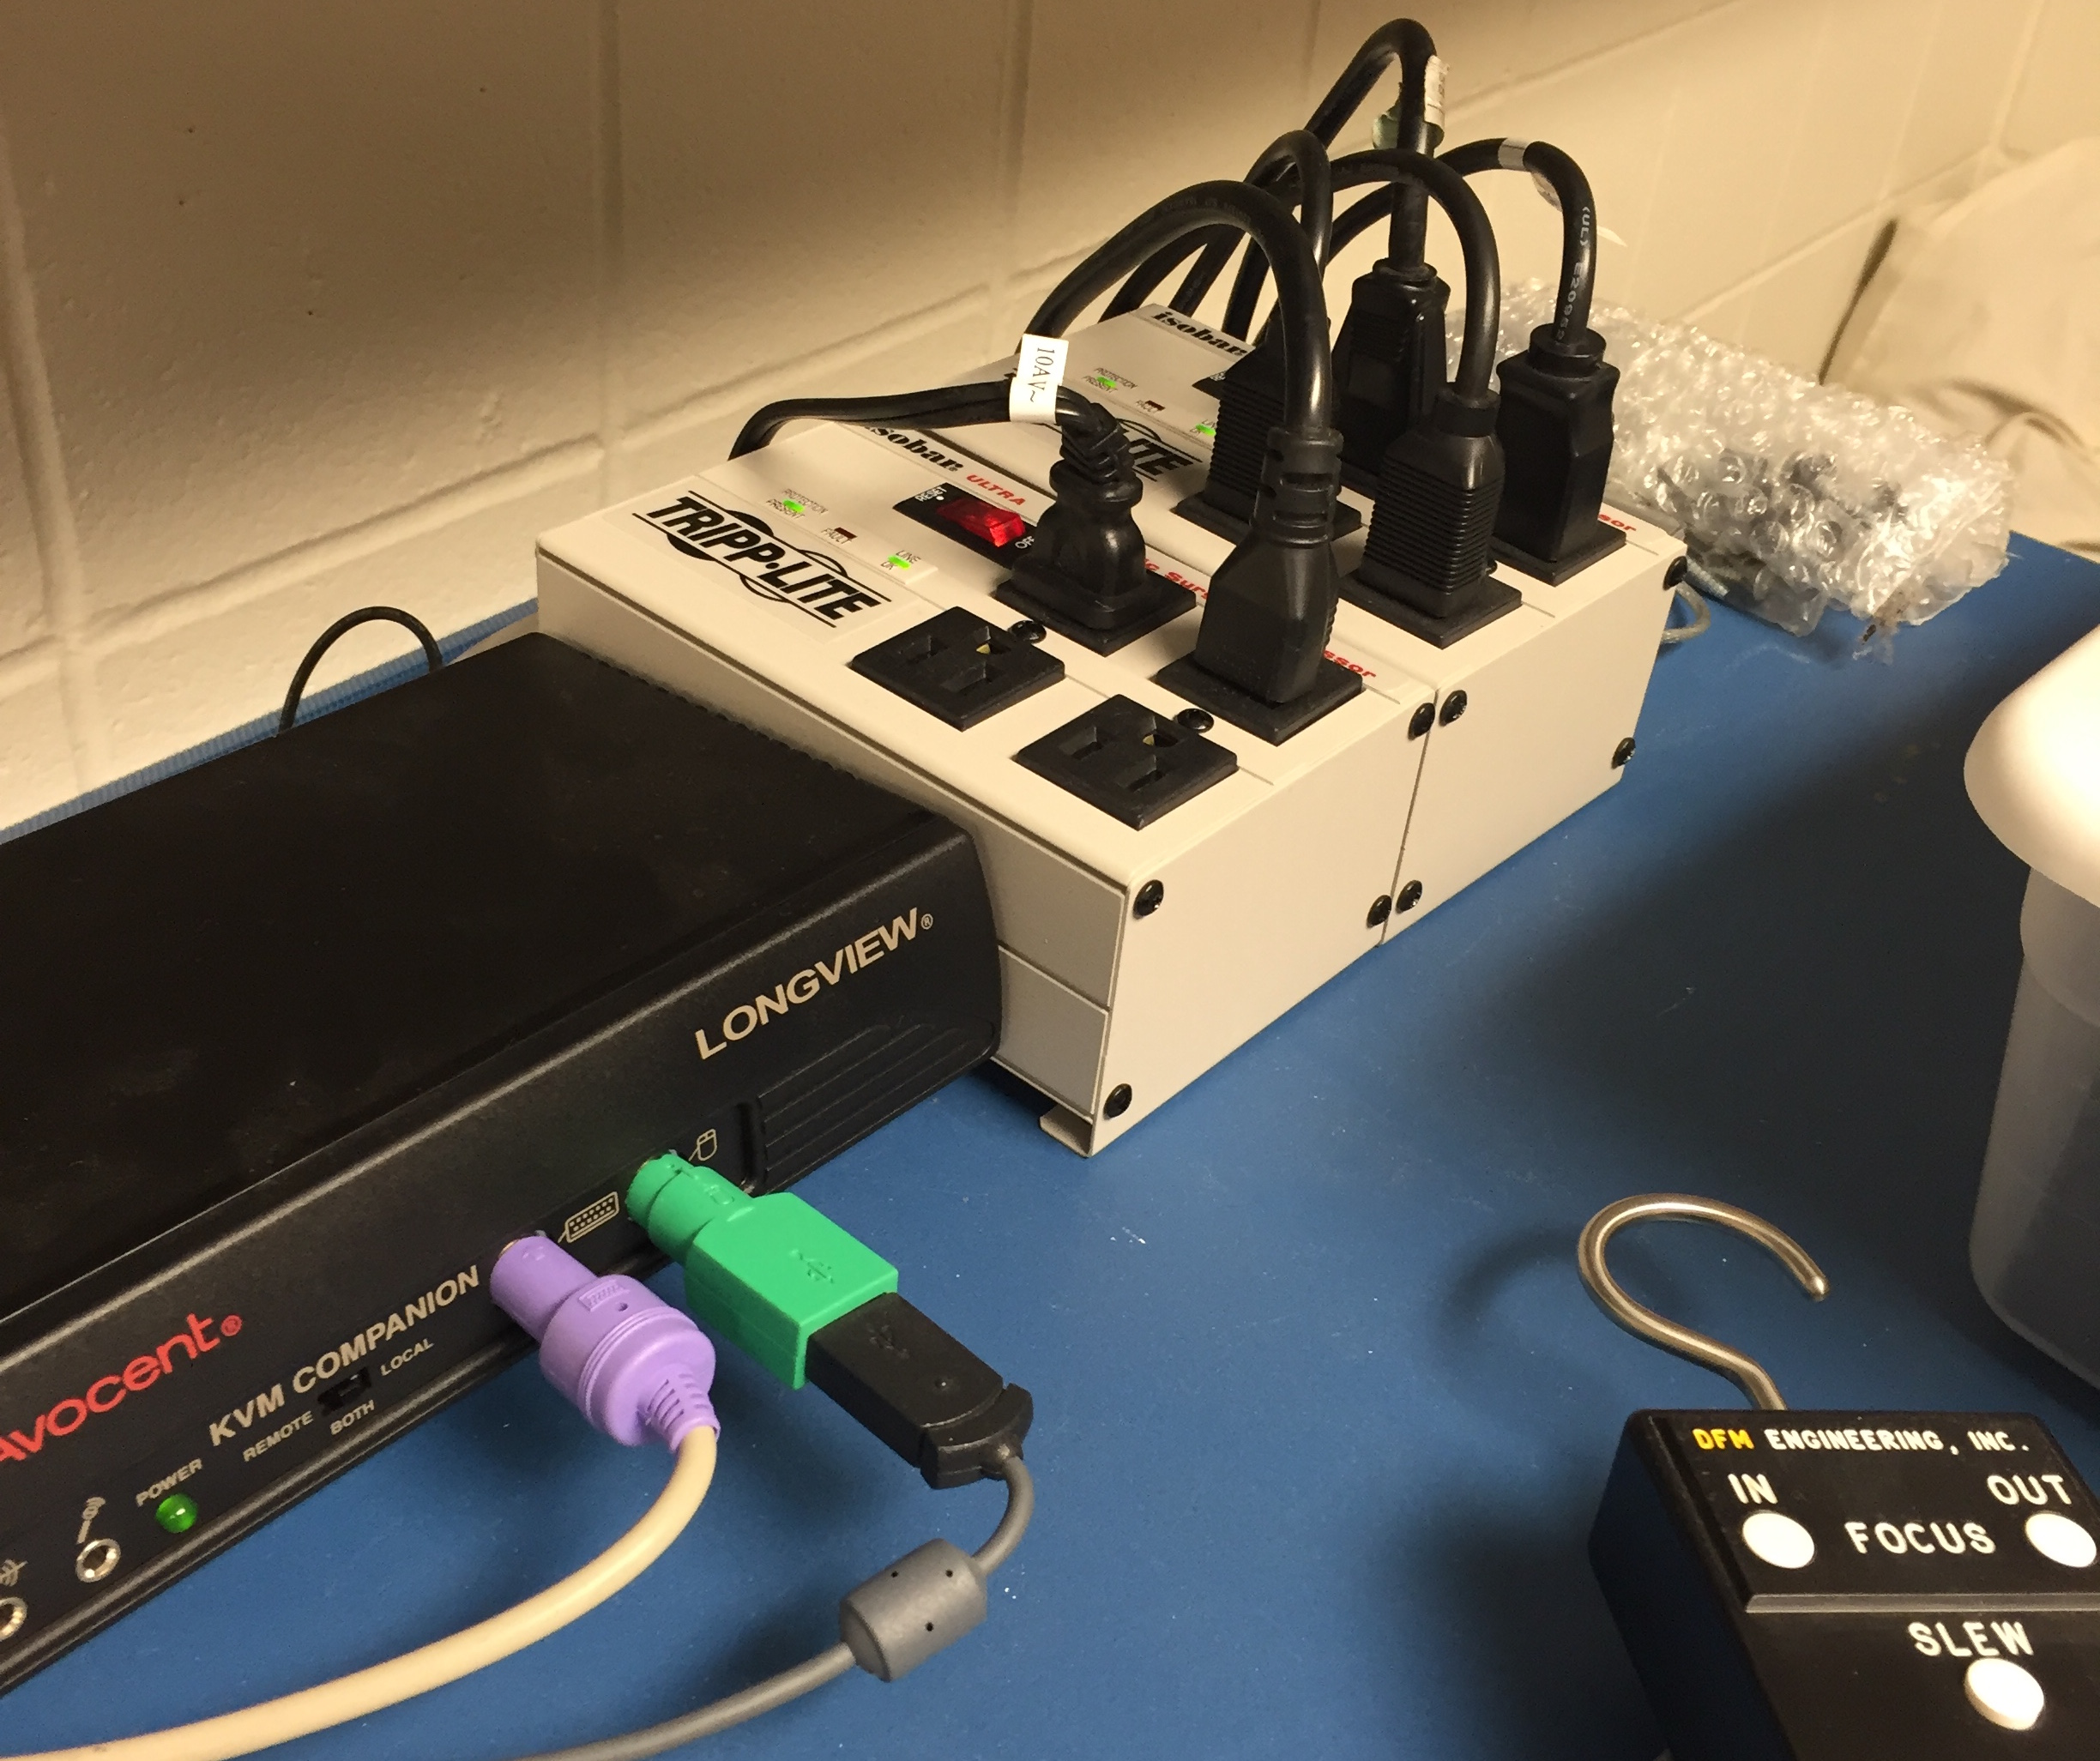
\includegraphics[width=2in,origin=c]{IMG_6751.JPG}
		\caption{Power strips}
	\end{minipage}
	\begin{minipage}{0.5 \linewidth}
		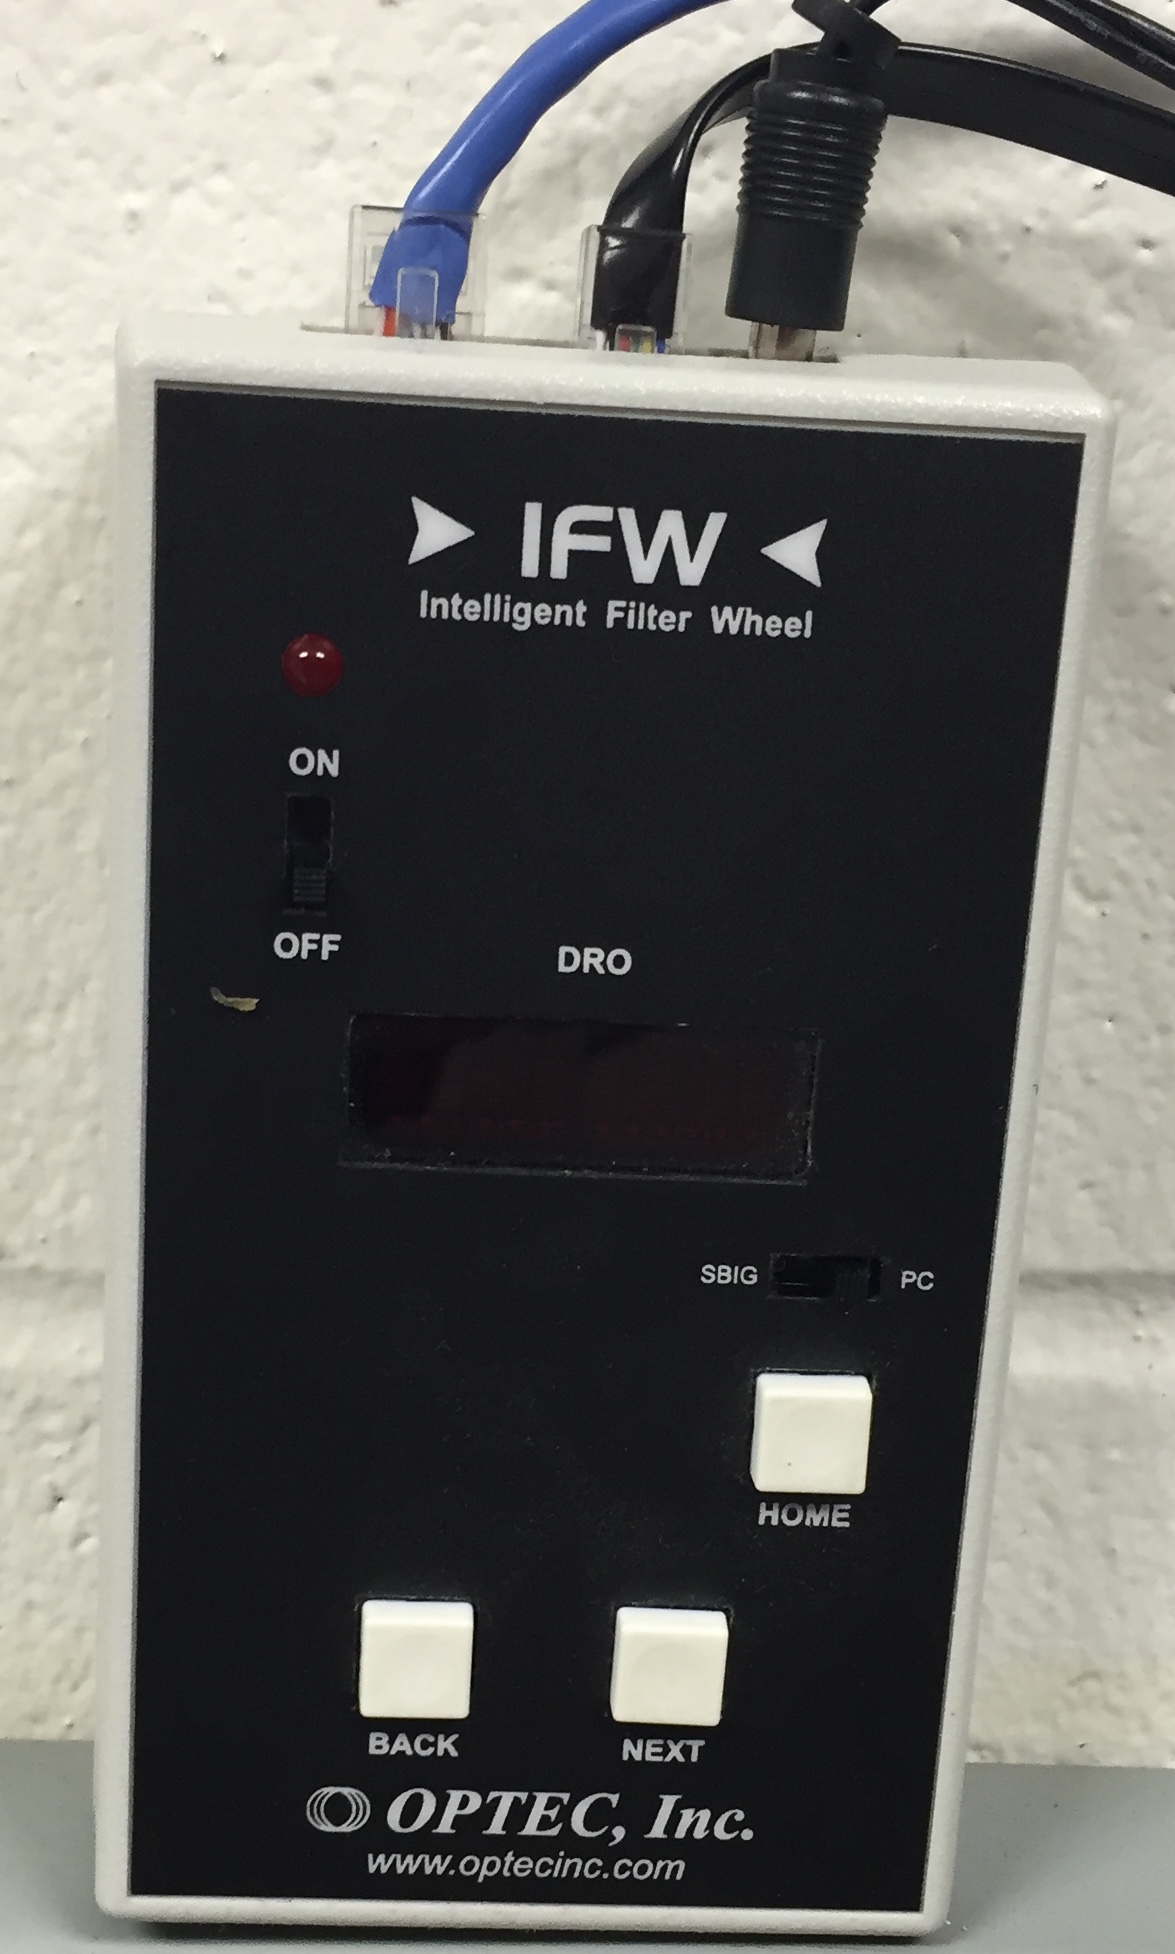
\includegraphics[width=2in,origin=c]{IMG_6752.JPG}
		\caption{Filter Wheel}
	\end{minipage}
\end{figure}


\end{document}
